\chapter{LED Patterns}

Who doesn't like a vibrant, scintillating display of colors? Be it shopping centers at the heart of the city's zeitgeist or the festivities at one's own abode, the on-and-off lighting patterns never fail to accentuate the appeal of the atmosphere. In this project, we will be using LEDs instead of light bulbs to generate aesthetic lighting patterns of our own.

\subsection*{Components}
\begin{table}[H]
    \centering
    \begin{tabular}{|c|l|c|}\hline
     \textbf{\#} & \textbf{Components} &  \textbf{Amount}\\\hline
     1 & Multi-color LEDs       &  24\\\hline
     2 & 470 $\Omega$ resistor   &  22\\\hline
     3 & Arduino UNO            & 1 \\\hline
     4 & Connecting wires       & - \\\hline
    \end{tabular}
\end{table}

\subsection*{Connections}

\begin{enumerate}[leftmargin=*]
    \item Connect 470 $\Omega$ resistors with the anode of all LEDs except those which are to be connected to pin 13 of Arduino.
    \item Connect other end of resistor of first 12 LEDs with pin 2 - 13 of Arduino.  .
    \item Connect other end of resistor of remaining  12 LEDS with LED's that are connected with Arduino such that LED 1 and 13 are connected to same pin on Arduino and so on. 
    \item Connect cathode of all LEDs with each other and then connect it to GND of Arduino.
\end{enumerate}

The circuit diagram shows how these components are to be connected:

	\begin{figure}[H]
	\centering 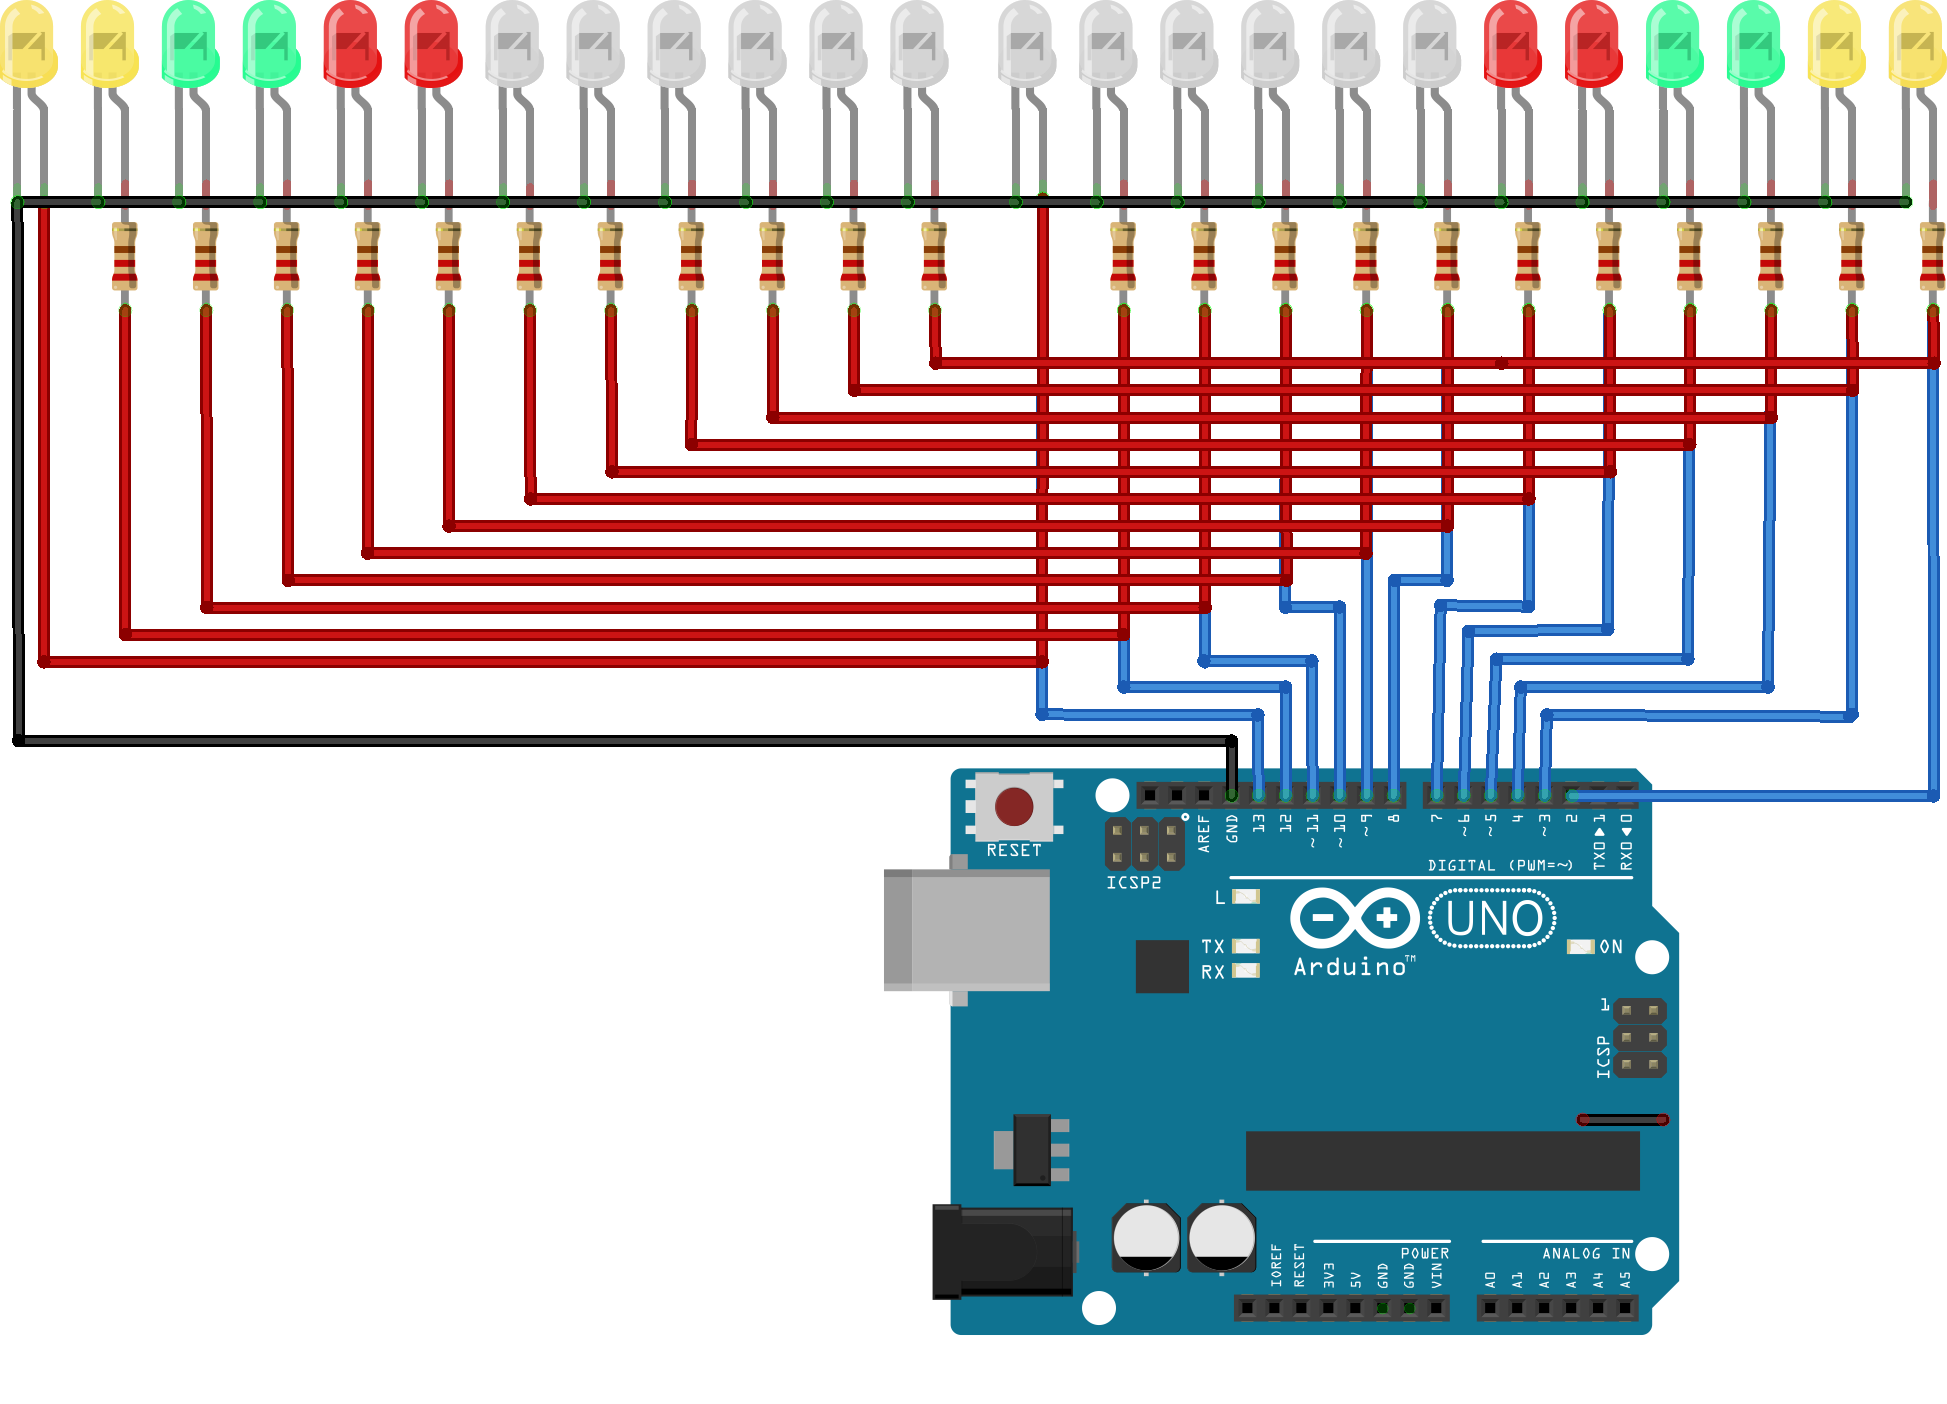
\includegraphics[width=0.6\linewidth]{Figures/recreational_exp/led pattern_bb.png}
	\caption{Circuit diagram}
	\end{figure}
	
\subsection*{Procedure}
\begin{enumerate}[leftmargin=*]
     \item Copy lst. \ref{list:led-pattern} to a new Arduino sketchbook. Upload the code to your Arduino board.
    \item Observe the changing patterns of LED lightning. 
    
\end{enumerate}
	
\begin{lstlisting}[language=Arduino, numbers=none, caption={Code for LED patterns}, captionpos=b, label={list:led-pattern}]
// variables to control patterns
int i,j;

//delay values
int D= 10, D1=200, D2=1000;

void setup() {
  
// There are 24 LEDs. 1st and last LED's are connected with same pin, 2nd and 2nd last LED.s are connected with same pin and so on. 
// We have 12 pins to control. Each pin is connected to 2 LED's.
// Setting all 12 pins as output

  pinMode(2, OUTPUT);
  pinMode(3, OUTPUT);
  pinMode(4, OUTPUT);
  pinMode(5, OUTPUT);
  pinMode(6, OUTPUT);
  pinMode(7, OUTPUT);
  pinMode(8, OUTPUT);
  pinMode(9, OUTPUT);
  pinMode(10, OUTPUT);
  pinMode(11, OUTPUT);
  pinMode(12, OUTPUT);
  pinMode(13, OUTPUT);
}

void pattern1 (void)
{
  // Pattern 1 Starts 
    for (j=1; j<=5; j++)
    {
      for(i=1; i<=13; i++)
      {
        digitalWrite(i, HIGH);
        delay(D);
        digitalWrite(i, LOW); 
      }
      for(i=13; i>=1; i--)
      {
        digitalWrite(i, HIGH);
        delay(D);
        digitalWrite(i, LOW); 
      }
    }
// Pattern 1 Ends.
}; 

void pattern2 (void)
{
  // Pattern 2 Starts 
   for(i=1; i<=13; i++)
   {
        digitalWrite(i, HIGH);
        delay(D1); 
   }

   pattern1();
          
    for (j=1; j<=5; j++)
    {
      for(i=1; i<=13; i++)
      {
        digitalWrite(i, LOW); 
      }
     delay(D1);           
      for(i=1; i<=13; i++)
      {
       digitalWrite(i, HIGH); 
      }
      delay(D1);
    }
    
   for(i=13; i>=1; i--)
   {
    digitalWrite(i, LOW);
    delay(D1);
   }
        pattern1();  
//pattern 2 ends
}; 

void pattern3 (void)
{
 //Pattern 3 start                                        
  for (j=1; j<=5; j++)
  {  
    for(i=7; i<=13; i++)
    {
      digitalWrite(i, HIGH); 
    }
    delay(D1);
    for(i=7; i<=13; i++)
    {
      digitalWrite(i, LOW);
    }
    for(i=1; i<=6; i++)
    {
      digitalWrite(i, HIGH); 
    }
    delay(D1);
    for(i=1; i<=6; i++)
    {
      digitalWrite(i, LOW);
    }
  }
//Pattern 3 Ends 
};


void loop() {
  pattern1();
  pattern2();
  pattern3();    
}
\end{lstlisting}

\begin{figure}[H]
	\centering 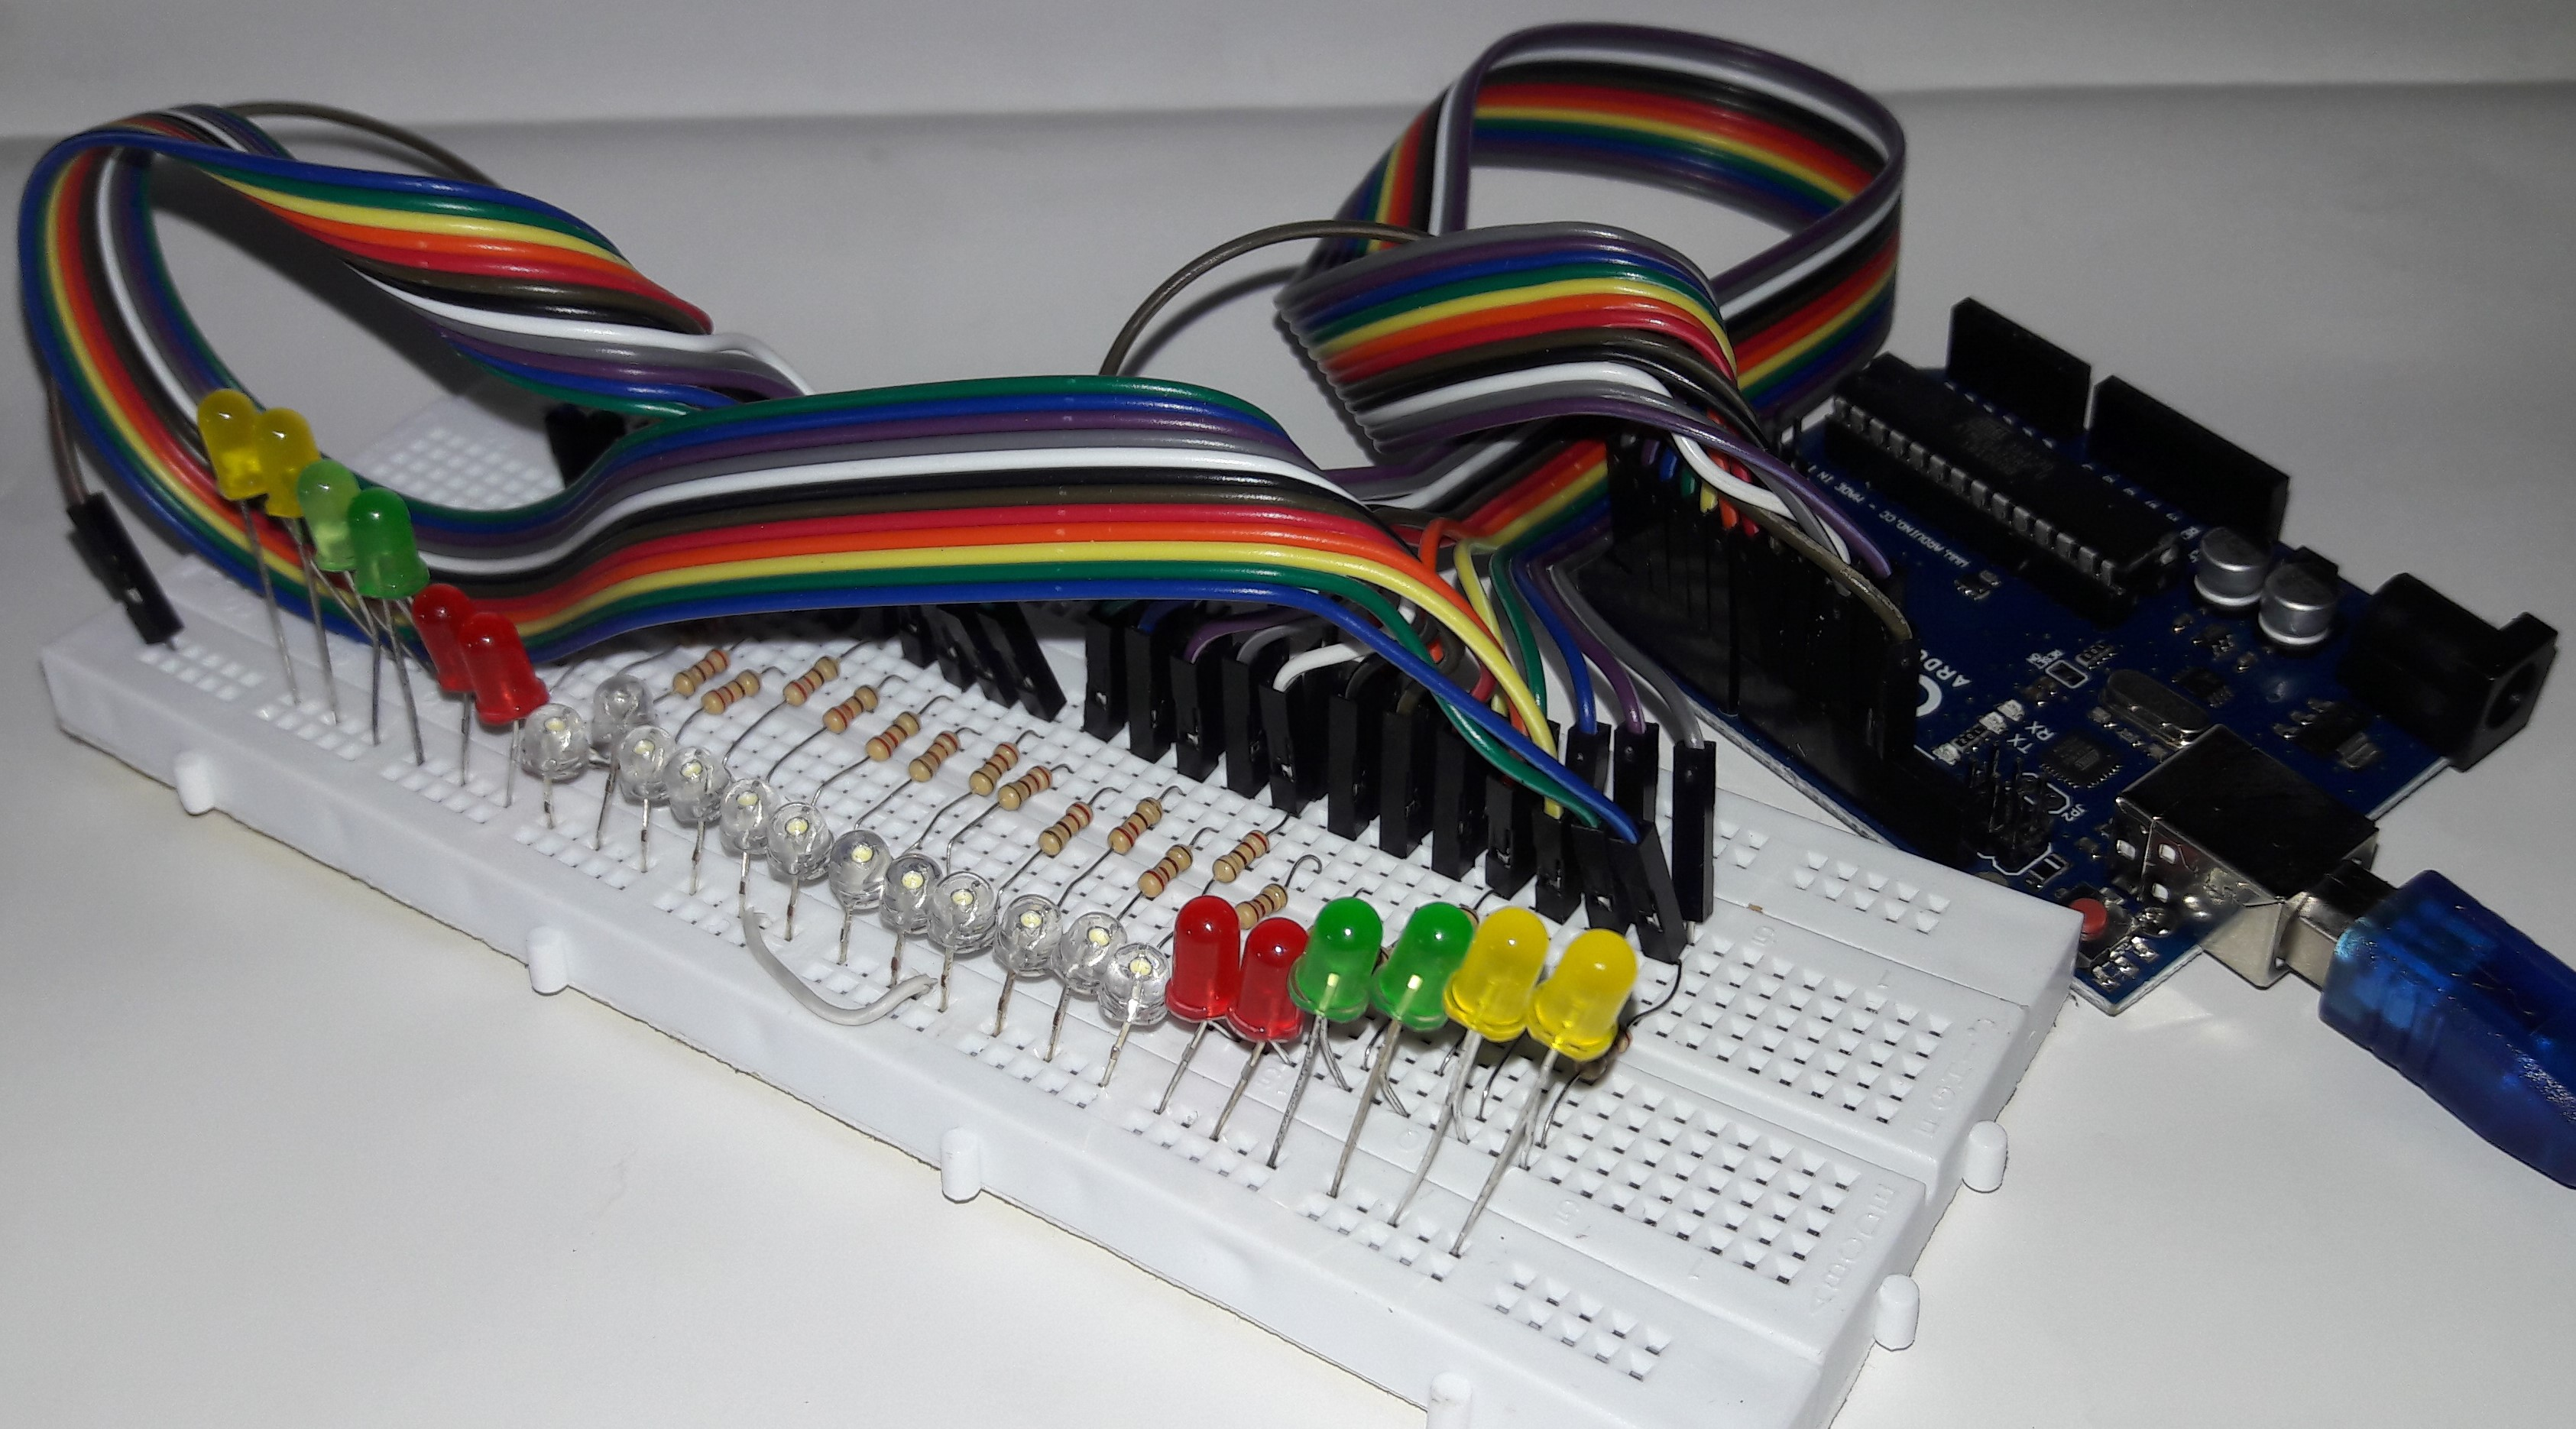
\includegraphics[width=0.7\linewidth]{Figures/recreational_exp/experiment_pics/led pattern.jpg}
	\caption{Hardware of the experiment}
\end{figure}